\documentclass{article}
\usepackage[utf8]{inputenc}
\usepackage[polish]{babel}
\usepackage{polski}
\usepackage{enumerate}
\usepackage{natbib}
\usepackage{graphicx}
\usepackage{geometry}
\usepackage{float}

\newgeometry{tmargin=2.5cm, bmargin=2.5cm, lmargin=2.5cm, rmargin=2.5cm}

\makeatletter
\newcommand{\linia}{\rule{\linewidth}{0.4mm}}
\renewcommand{\maketitle}{\begin{titlepage}
    \vspace*{1cm}
    \begin{center}
    Politechnika Wrocławska\\
    AiR ARR\\
 Projekt zespołowy
    \end{center}
      \vspace{3cm}
    \begin{center}

     \LARGE \textsc {\@title}
         \end{center}
     \vspace{1cm}

    \begin{center}
    \textit{ Autorzy:}\\
   \textit{\@author}
     \end{center}
      \vspace{1cm}

     \begin{center}

    Prowadzący:
  dr inż. Krzysztof Arent
    \end{center}

    \vspace*{\stretch{6}}
    \begin{center}
    \@date
    \end{center}
  \end{titlepage}
}
\makeatother
\author{Beata Berajter\\
Dawid Brząkała\\
Dorota Gidel\\
Katarzyna Wądrzyk\\
Ada Weiss\\
Małgorzata Witka-Jeżewska\\
 }
\title{SensGlove}

\begin{document}

\maketitle
\newpage
\tableofcontents
\newpage


\section{Wymagania użytkownika i specyfikacja funkcjonalności}
Użytkownik powinien mieć możliwość założenia sprzętu, to znaczy rękawiczki sensorycznej (zawierającej czujniki ugięcia i nacisku) a także czujników miopotencjałów, oraz uruchomienia programu służącego do odbioru ich. Wtedy, po poprawnym podłączeniu się, użytkownik powinien mieć możliwość podglądu w czasie rzeczywistym wykonywanych ruchów. W przypadku poprawnego działania każdego z czujników użytkownik powinien mieć możliwość utworzenia odpowiedniego folderu i zapisania do niego wyników odczytów z czujników od momentu wciśnięcia przycisku START do zdefiniowanej wcześniej długości czasu. Użytkownik powinien mieć możliwość wykonania i zapisu dowolnej ilości pomiarów oraz stworzenie dowolnej ilości folderów oznaczających kolejne gesty.

\section{Kryteria ewaluacji}
Komponenty powinny działać każde z osobna oraz współdziałać jako kompletne stanowisko do pobierania sygnałów i biosygnałów. Użytkownik powinien mieć możliwość wykonywania ruchów w obrębie przynajmnie jednego metra od stanowiska. Rękawiczka pomiarowa powinna mieć umieszczone czujniki w taki sposób, aby nie ograniczała ruchów ani tym bardziej nie krępowała ich. Pomiary przesyłane mają być w czasie rzeczywistym, a ich podgląd zapewnić ma program wizualizujący je.

\section{Rozpoznanie możliwości wykonania bazy sprzętowo-programowej}

\subsection{Projekt oparty na płytce deweloperskiej STM32F3Discovery}
ZALETY:
\begin{enumerate}
    \item Duża ilość wejść analogowych.
\item Możliwość podłączenia wszystkich czujników do jednej płytki.
    \item Spora ilość informacji na temat płytki i jej obsługi dostępna w bibliotekach oraz poprzez Internet.
\item Możliwość rozpoczęcia prac w ciągu dwóch tygodni w zależności od szybkości dostawy.
\end{enumerate}
WADY:
\begin{enumerate}
    \item Szeregowy przesył danych, przez co mogą powstać problemy podczas przesyłania ich - opóźnienia.
\end{enumerate}
\subsection{Projekt oparty na dostępnej już karcie NI PCI-6034E}
ZALETY:
\begin{enumerate}
    \item Możliwość przesyłania równolegle 16 sygnałów jednocześnie.
    \item Gotowy program korzysający ze sterownika NiDAQ Mx oraz zawierający bibliotekę obsługującą kartę.
\item Gotowe stanowisko pomiarowe do EMG i MMG.
\item Możliwość współpracowania z programem Matlab. 
\item Wsparcie techniczne.
\end{enumerate}
WADY:
\begin{enumerate}
    \item Konieczność podporządkowania się już stworzonym rozwiązaniom.
\end{enumerate}
Istenieje również możliwość korzystania z nowo zakupionej karty przetworników, niestety na chwilę obecną nie posiadamy jej dokładnej nazwy, przez co niemożliwym jest dokonanie rozeznania w jej przypadku.


\section{Podział na komponenty, architektura i kryteria ewaluacji komponentów}
\subsection{Rękawiczka sensoryczna}
Osoby przydzielone do zadania: Dorota Gidel, Katarzyna Wądrzyk.
\subsubsection{Wymagania użytkownika}
Na rękawiczce powinno znajdować się tyle sensorów, aby pomiary były jak najdokładniejsze, lecz nie za dużo, aby nie przyćmić potrzebnych danych. Zaproponowane zostało zamontowanie sensorów nacisku (co najmniej 5 - jeden na jeden palec) oraz sensorów ugięcia (co najmniej 5 - jeden na jeden palec). Umiejscowienie czujników powinno być na tyle odpowiednie, aby nie utrudniały ani ograniczały one ruchów palców. Sama rękawiczka powinna być dopasowana do dłoni użytkownika, tutaj proponowane zostało wykonanie rękawiczki w dwóch rozmiarach.
\subsubsection{Funkcjonalność}
Do projektu zostanie użyta rękawiczka do biegania, na dłoń prawą. Zapewni ona dobrą zdolność manualną oraz skuteczne dopasowanie do dłoni. Rękawiczka będzie tylko w jednym rozmiarze ze względu na dodatkowe nakłady czasu i pieniędzy potrzebne do jej wykonania. Przez wzgląd na skład grupy wykonawczej, rękawiczka będzie w rozmiarze małym, tj. S (7).\\
Planowane jest użycie 10 czujników nacisku (na każdym palcu po dwa, od strony wewnętrznej dłoni), których rezystancja maleje wraz ze wzrostem siły nacisku oraz 5 czujników ugięć (po jednym na każdy palec, od strony zewnętrznej dłoni), których rezystancja rośnie wraz ze zwiększeniem kąta ugięcia. Czujniki będą przyszyte do rękawiczki, a w miejscach najbardziej narażonych na zahaczenia, takie jak koniec palca, przyklejone klejem. \\

\begin{figure}[h!]
\centering
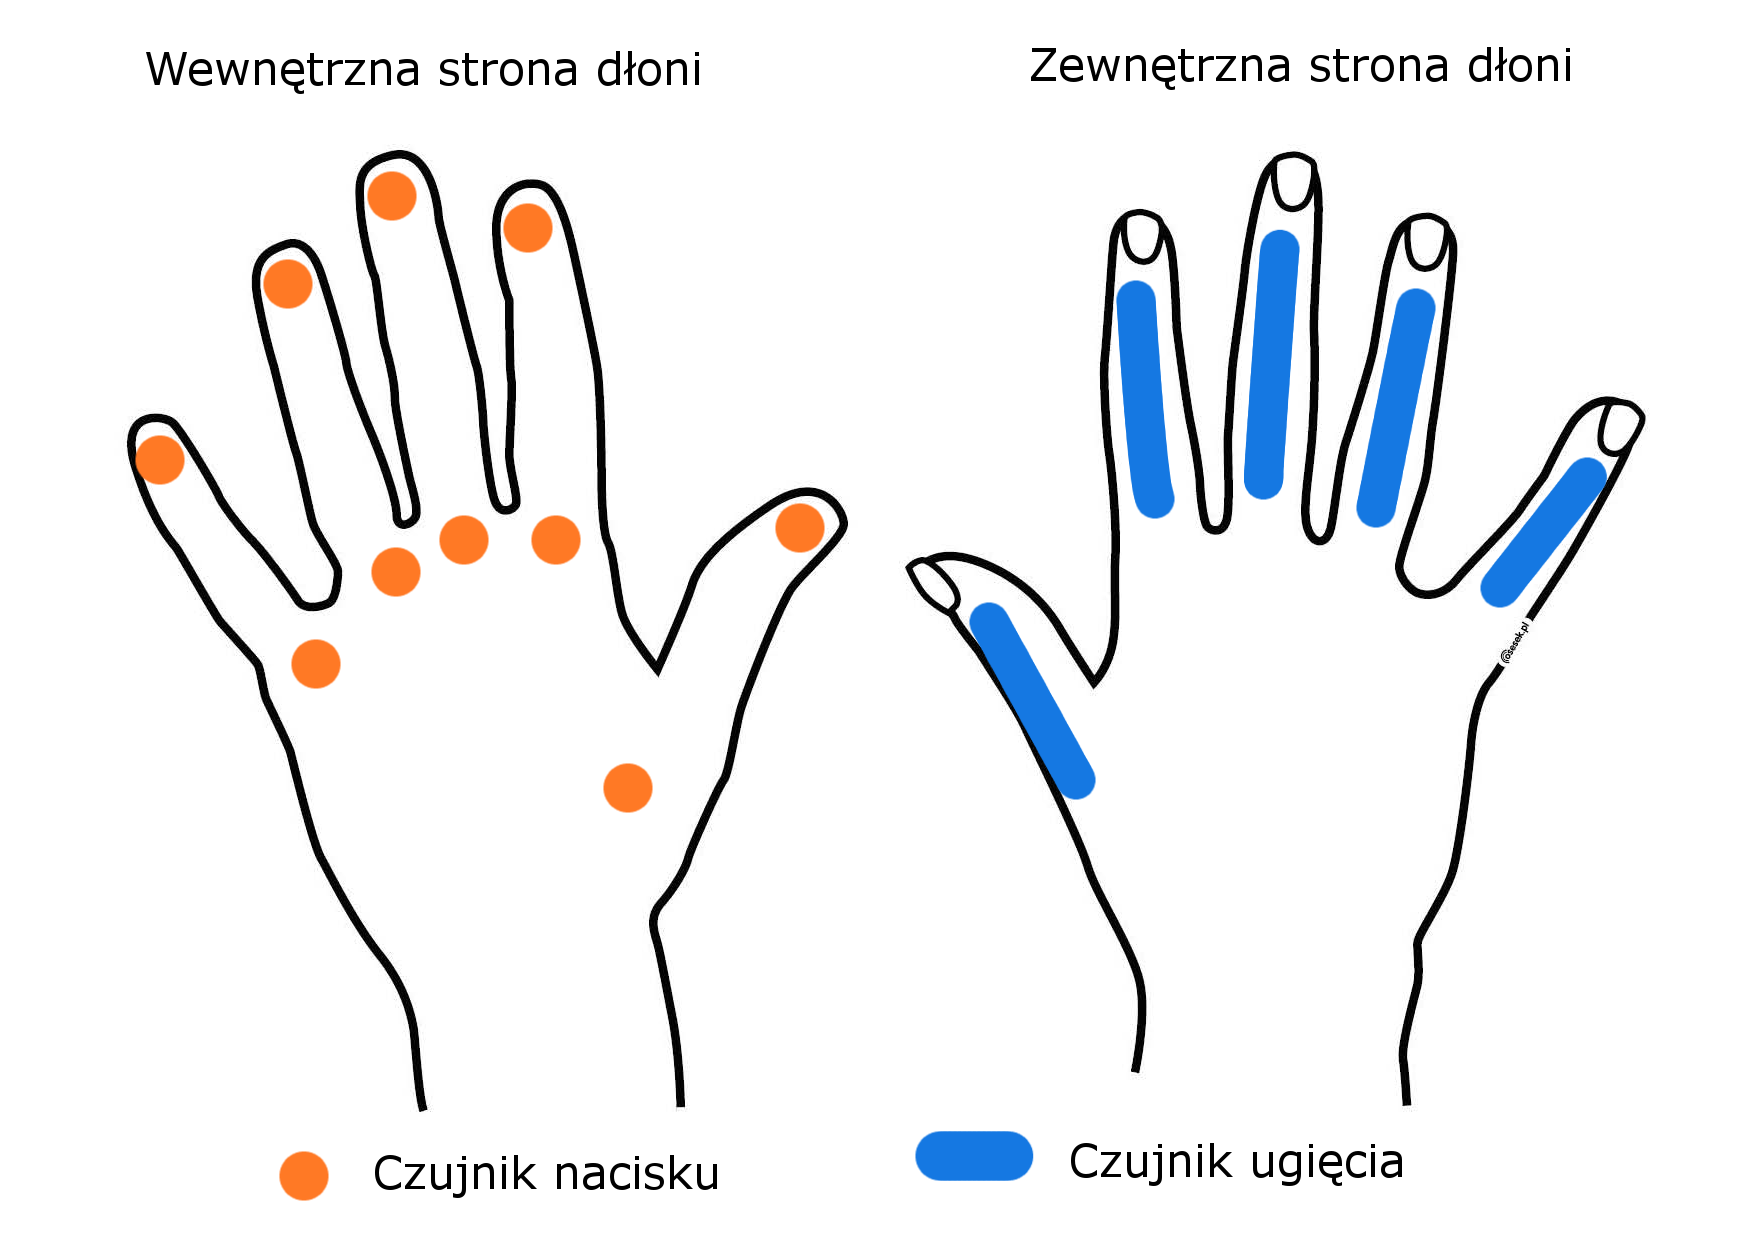
\includegraphics[width = 10cm]{czujniki.png}
\caption{Układ czujników na rękawiczce}
\label{fig:rozmieszczenie_czujników}
\end{figure}

\subsubsection{Kryteria ewaluacji}
Skończona rękawiczka pozwalać będzie na wykonywanie ruchów ograniczonych jedynie rozmiarem dłoni użytkownika (dostępny będzie tylko jeden rozmiar rękawiczki) oraz przewodów łączących czujniki z płytką. Będzie ona odporna na upadki z niewielkich wysokości oraz na wielokrotne ściąganie i zakładanie jej. Czujniki będą przymocowane tak, aby podczas energicznego machania pozostały one na swoim miejscu.\\
Sprawność czujników sprawdzona będzie poprzez zmierzenie miernikiem rezystancji. Przy zgięciu palca rezystancja czujnika ugięcia będzie wzrastać, a podczas nacisku rezystancja na czujnikach będzie maleć. Po podłączeniu wszystkiego do płytki sprawdzone będzie czy wysyłany jest sygnał z czujników. Celem tego testu będzie sprawdzenie czy połączenie z płytką jest poprawne.
\subsubsection{Podział zadań}
Gidel Dorota:
\begin{itemize}
    \item przyszycie czujników do rękawiczki
    \item przyszycie okablowania do rękawiczki
\end{itemize}
Wądrzyk Katarzyna:
\begin{itemize}
    \item kupno czujników, rękawiczki oraz okablowania
    \item montaż czujników do przewodów
\end{itemize}
\subsubsection{Potrzebne elementy i kosztorys}
Do rękawiczki (rękawiczki do biegania, czarnej KALENJI) przymocowane będą następujące czujniki:
\begin{itemize}
    \item Czujnik nacisku 5mm FSR400, short tail
    \item Czujnik zgięcia FS7954 55mm
\end{itemize}
Ich odprowadzenia do płytki będą zrealizowane poprzez przewód 2x0.5mm biały YTDY.
Same czujniki przyłączone będą za pomocą lutów do przewodów.
Dokumentacje czujników:

\begin{itemize}
  \item czujnik ugięcia: electropark.pl/attachment.php?id\textit{\_}attachment=850
  \item czujnik nacisku: electropark.pl/attachment.php?id\textit{\_}attachment=1834

\end{itemize}

\begin{table}[ht!]
\centering
\caption{Kosztorys elementów do rękawiczki sensorycznej}
\begin{tabular}{|c|l|c|c|c|}
\hline
    numer & nazwa & ilość & cena jednostkowa [zł] & cena całościowa [zł] \\
 \hline
    1 & czujnik ugięcia & 5 & 40,99 & 204,95 \\
    2 & dotykowy czujnik nacisku & 10 & 25,26 & 252,60 \\
    3 & rękawiczka & 1 & 10,99 & 19,99 \\
    4 & przewody & 3 & 0,50 & 1,50 \\
    \hline
    5 & suma & & & 479,04\\
    \hline
\end{tabular}
\label{tab:rekawiczka}
\end{table}

% potrzebny sprzęt i elementy, konkretne  czujniki, ich liczba, ich dokumentacja, cena (pamiętajcie o wyborze rękawiczki!), czas na uzyskanie ich
% wstępna koncepcja rozmieszczenia elementów, opis słowno-muzyczny
% schematy ideowe, sposób podłączania, ilość wejść i wyjść, zakresy działania z dołączonej dokumentacji
% poszczególne zadania, jakie trzeba wykonać i kto je zrobi, najlepiej przypisane do jednej osoby
% sposób testowania, czy działa, rozpisanie na poszczególne kryteria
% napisanie co będzie oznaczać wykonania zadania poprawnie
\subsection{Interfejs sprzętowy}
% potrzebny sprzęt i elementy, ich liczba, ich dokumentacja, cena, czas na otrzymanie ich
% wstępna koncepcja rozmieszczenia elementów, opis słowno-muzyczny
% schematy ideowe, sposób podłączania, ilość wejść i wyjść, zakresy działania z dołączonej dokumentacji
% potrzebne biblioteki
% BARDZO WAŻNE, kryterium sprawdzające, czy odczyty są zsynchronizowane!
% suma kontrolna
% poszczególne zadania, jakie trzeba wykonać i kto je zrobi, najlepiej przypisane do jednej osoby
% propozycja wysyłania danych
% sposób testowania, czy działa, rozpisanie na poszczególne kryteria
% napisanie co będzie oznaczać wykonania zadania poprawnie
Osaby przydzielone do zadania: Beata Berajter i Dawid Brząkała. \\
Interfejs będzie miał za zadanie odczyt wartości z czujników zgięcia i nacisku z rękawiczki oraz czujników biopotencjałów i przesyłał je w odpowiednim formacie do komputera poprzez kabel USB i wirtualny port COM. Sygnały z czujników zostaną wzmocnione przez układ ze wzmacniaczami operacyjnymi, który również zadba o to, aby wartości sygnałów wyjściowych mieściły się w zakresie pracy przetwornika ADC mikrokontrolera (0 - 3.3V). Zasilanie układu pochodzić będzie ze złącza USB.
\subsubsection{Schemat ideowy}
\begin{figure}[h!]
\centering
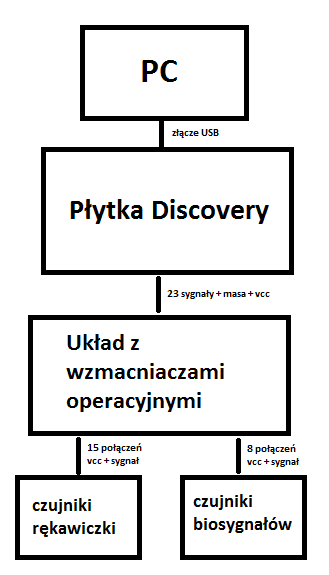
\includegraphics[width=6cm]{schemat_ideowy_interfejsu.png}
\label{fig:interfejs}
\caption {Schemat ideowy interfejsu sprzętowego}

\end{figure}
Schemat przedstawiony jest na rysunku 2.
% plik "schemat ideowy interfejsu.png" nie wiem jak się wstawia obrazki



\subsubsection{Potrzebne elementy}

Lista elementów wraz z przewidywanymi kosztami została przedstawiona w tabeli \ref{tab:interfejs}.
\begin{table}[th!]
\centering
\caption{ Lista potrzebnych elementów}

\begin{tabular}{|r|l|l|} \hline

element & ilosc & cena\\ \hline
rezystory 10kOhm & 20 & 0.60zł/10szt \\
listwa kołkowa 1x40 pin & 1 & 0.69zł/szt \\
listwa kołkowa 2x40 pin & 1 & 1.00zł/szt \\
wzmacniacz operacyjny TL084 & 6 & 8,34zł/szt \\
dioda zenera 3V3 & 24 & 0.12zł/szt \\
STM32F3 - DISCOVERY - Cortex-M4F & 1 & 102.90zł/szt \\
laminat światłoczuły 100x160x1.5mm dwustronny + & 1 & 15.00zł/szt \\\hline % jeśli wytrawiamy sami, jak będziemy zamawiać będzie trzeba zmienić
razem & & 131.41zł \\\hline
\end{tabular}
\label{tab:interfejs}
\end{table}


\subsubsection{Kryteria ewaluacji}
Aby sprawdzić poprawność odczytu sygnałów przez przetworniki ADC czujniki będą symulowane poprzez potencjometry, a uzyskane wyniki przesłane do komputera. Poprawność samej transmisji sprawdzona zostanie poprzez wysyłanie zaprogramowanych wcześniej przykładowych wiadomości i odczytywanie ich w komputerze poprzez program do monitowania portów COM.

\subsection{Program do akwizycji danych}
Osoby przydzielone do zadania: Ada Weiss, Małgorzata Witka-Jeżewska\\
Zadaniem programu będzie odczyt danych przesyłanych z mikrokontrolera z portu USB komputera. Użytkownik po uruchomieniu programu będzie miał możliwość rozpoczęcia procesu akwizycji danych. Dane będą wczytywane przez określony czas (prawdopodobnie 2s jak w dotychczasowych badaniach miosygnałów z przedramienia, co pozwoliłoby na synchronizację tych pomiarów) odszyfrowywane i przesyłane do programu do tworzenia wizualizacji rękawiczki i danych z sensorów z wykorzystaniem socketów. Dodatkowo program będzie umożliwiał użytkownikowi wybór typu ruchu który jest obecnie wykonywany. Każdorazowo po wykonanym pomiarze użytkownik będzie musiał zdecydować czy dany pomiar zapisać czy go odrzucić. W przypadku zapisu uruchomiony będzie skrypt. Oprogramowanie będzie tworzone w systemie Linux z użyciem Qt kreatora.
\subsubsection{Format danych}
Dane odbierane będą w postaci stringa z zakodowanymi heksadecymalnie wartościami odczytu z kolejnych czujników. Do sprawdzenia poprawności przesyłu wykorzystana będzie suma kontrolna.
\subsubsection{Kryteria ewaluacji}
Symulacja danych wejściowych: \\
Zaprogramujemy płytkę STM32L476G Discovery tak aby nadawała przykładowe dane w ustalonym przez nas formacie i podłączymy ją do USB komputera.  \\
Poprawność danych wyjściowych:\\
Wykorzystamy również przykładowy program klient odbierający dane wysyłane z napisanego programu (serwera) w celu ocenienia poprawności przesyłania danych.\\

\subsubsection{Schemat ideowy}
\begin{figure}[h!]
\label{fig:program}
\centering
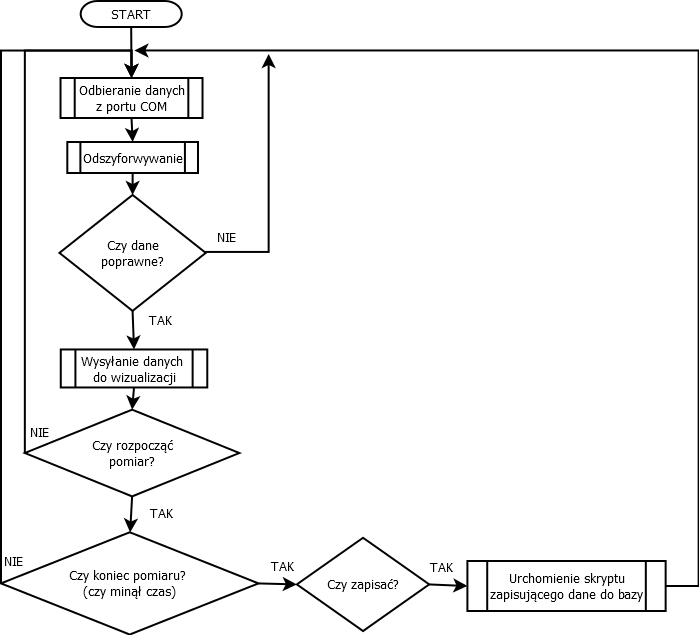
\includegraphics[width=10cm]{programdia.png}
\caption{Schemat ideowy działania programu}
\end{figure}
\subsubsection{Podział zadań}

Ada Weiss:
\begin{itemize}
\item odczytywanie danych z portu COM
\item przesyłanie danych za pomocą gniazda
\end{itemize}
Małgorzata Witka-Jeżewska:
\begin{itemize}
    \item stworzenie odpowiednich okien i odpowiednich metod z nimi stowarzyszonych
\end{itemize}


% potrzebne biblioteki
% schematy ideowe
% klasy
% podział pracy
% protokół zbierania danych
% testy i kryteria ewaluacji
% tworzenie bazy danych
\subsection{Baza danych}
Osoby przydzielone do zadania: Beata Berajter, Dorota Gidel
\subsubsection{Wymagania użytkownika}
Stworzenie bazy danych ma na celu zebranie oraz odpowiednie uporządkowanie zebranych danych pomiarowych. Baza powinna być utworzona w sposób przemyślany i logiczny.
\subsubsection{Funkcjonalność}
Dane zawierające odczyty z czujników i wartości miopotencjałow zapisywane będą w formie plików tekstowych. Zdecydowano się na tekstowy format bazy danych, ponieważ istnieje prawdopodobieństwo, że będą one przekazane innym jednostkom, które preferują taką formę i w ten sposób najlepiej się będzie można zsynchronizować. Baza danych zawierać będzie katalogi odpowiadające osobom badanym (wykonującym eksperymenty w rękawiczce). W każdym z tych katalogów znajdować będą się podkatalogi z wykonywanymi typami badanych ruchów/chwytów. Z kolei w tych podkatalogach tworzone będą kolejne trzy podkatalogi, jeden zawierający dane z elektrod, drugi z czujników nacisku, trzeci z czujników zgięcia na rękawiczce sensorycznej. W tych folderach znajdować się będą pliki tekstowe z pomiarami. Każdy plik tekstowy zorganizowany będzie w formie macierzy. Zakładając że pomiar będzie trwał 2 sekundy, a odczyt z czujników i elektrod będzie następował z częstotliwością 1kHz, plik taki będzie zawierał 2000 lini (1000*2). Ilość kolumn w danym pliku to liczba dostępnych czujników/elektrod z których pobieramy dane. Planowane jest 8 elektrod, 10 czujników nacisku i 5 czujników zgięcia, więc pliki te odpowiednio zawierać będą macierze 2000 wierszy i 8 kolumn, 2000 wierszy i 10 kolumn, 2000 wierszy i 5 kolumn. Każdy kolejny zapisany pomiar (2 sekundowy) zapisywany będzie w pliku którego nazwa będzie informować o tym który jest to pomiar z kolei (dla danej osoby i typu ruchu) i dokłądnej dacie zapisania pomiaru do bazy\\
Baza danych będzie współpracować z programem do akwizycji danych. Napisana zostanie funkcja, która wywoływana będzie przez ten program. Jej celem będzie, przy podanych odpowiednich argumentach, utworzenie folderów i pliku tekstowego z pomiarami w odpowiednim miejscu w bazie danych. Powstanie również funkcja pozwalająca na odnalezienie pożądanego pomiaru, wykonanego na danej osobie i podanej dacie.

\begin{figure}[ht!]
\label{fig:baza_danych}
\centering
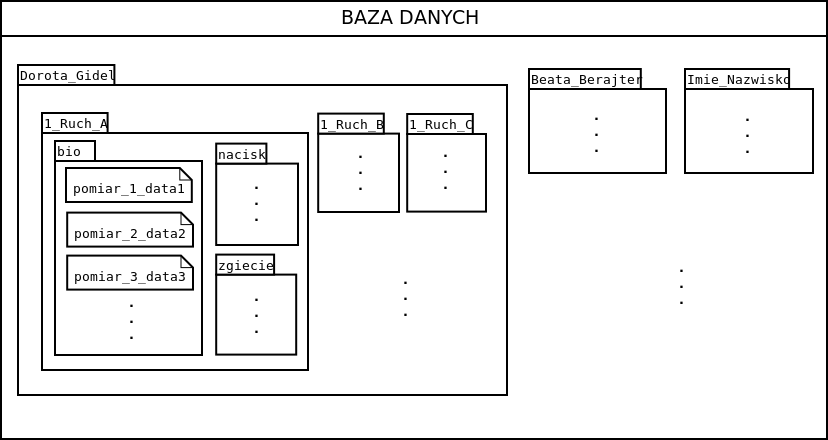
\includegraphics[width=14cm]{baza_danych.png}
\caption {Schemat struktury bazy dancyh}
\end{figure}
\subsubsection{Kryteria ewaluacji}
Do sprawdzenie poprawności działania bazy danych, zostanie wywołana funkcja obsługi bazy z przykłądowymi argumentami i danymi z czujników. Zarówno wejściowym, jak i wyjściowym efektem są pliki tekstowe. Zostaną utworzone przykładowe, testowe pliki, dzięki którym, będzie można porównać oraz sprawdzić poprawność przetworzonych danych.
\subsubsection{Podział zadań}
Beata Berajter:
\begin{itemize}
    \item funkcja/skrypt wyszukujący pomiar z bazy danych
\end{itemize}
Dorota Gidel:
\begin{itemize}
    \item funkcja/skrypt zapisujący pomiar do bazy danych
\end{itemize}

\subsection{Wizualizacja danych}
Osoby przydzielone do zadania: Dorota Gidel, Katarzyna Wądrzyk
\subsubsection{Wymagania użytkownika}
Od aplikacji wymagane jest aby w przejrzysty sposób wyświetlała zbierane dane z rękawiczki sensorycznej na modelu dłoni w 3D. Oczekiwane jest aby tworzony był wykres danych w czasie rzeczywistym (z możliwością rozróżnienia na poszczególne czujniki). Wymagane jest także aby po najechaniu myszką na konkretny obszar na modelu dłoni, wyświetlone zostały dokładne dane o tym punkcie (wartość siły, zgięcia).
\subsubsection{Funkcjonalność}
Odczyt informacji przez aplikację odbywa się poprzez użycie socketów, dane będą przesyłąne z programu do akwizycji danych. Ciągły strumień danych będzie obierany i przetwarzany z częstotliwością około 25Hz.\\
Aplikacja obrazować będzie dane pobierane z rękawiczki sensorycznej na modelu ręki 3D, zmieniając ułożenie palców w zależności od dostarczonych pomiarów. Dodatkowo odczyty z czujników nacisku prezentowane będą poprzez zmianę koloru opuszków palców w zależności od siły. Przy maksymalnej sile nacisku na wizualizacji będzie odpowiadał kolor czerwony a minimalnej sile odpowiadać będzie kolor zielony. Zamodelowana zostanie prawa ręka.\\
Program umożliwiać będzie prezentację zmiany odczytów danych na wykresie. Planowany podstawowy zakres informacji obejmuje 30s. \\
W celu uzyskania przejrzystego interfejsu, zastosowane zostanie grupowanie względem typu czujnika. Zrealizowane to zostanie poprzez zakładki, które umożliwiaią szybki dostęp do pożądanych informacji. \\
Program będzie tworzony w Qt5 na Linuxie.
\subsubsection{Kryteria ewaluacji}
Działanie programu sprawdzone będzie pod kątem odbierania sygnału z rękawiczki oraz poprawnego wyświetlania danych na modelu 3D. \\
Gdy wysłany zostanie sygnał maksymalnego nacisku z czujnika na palcu wskazującym program go odczyta oraz wyświetli kolor czerwony na wizualizacji. Gdy zgięty zostanie dany palec u ręki, palec na modelu w programie również zostanie zgięty. Gdy kąty zgięcia oraz kolory nacisku będą się zgadzać, znaczyć to będzie, że aplikacja działa poprawnie. Dane te mogą być sztucznie symulowane i wysyłane do programu by istniała możliwość testowania bez istnienia poprawnie działających komponentów systemu.
\subsubsection{Podział zadań}
Gidel Dorota:
\begin{itemize}
    \item tworzenie klas zakładek
    \item tworzenie modelu dłoni
    \item tworzenie funkcji ruchu dłoni
    \item tworzenie aktywnych obszarów na dłoni
\end{itemize}
Wądrzyk Katarzyna:
\begin{itemize}
    \item tworzenie okna głównego przycisków
    \item tworzenie klas wykresów
    \item tworzenie wykresów
    \item tworzenie obsługi odczytu danych
\end{itemize}
\end{document}
